\documentclass[11pt]{article}
\newcommand\tab[1][1cm]{\hspace*{#1}}
\usepackage{graphicx}
\usepackage{float}

\begin{document}
	\title{Ticket Salad Application User Manual}
	\date{Hackermen}
		
	\author{Tristan Joseph \\ Jarryd Baillie \\ Brandon Teixeira \\ Gift Mothusi \\ Thomas Honiball }

		
	\maketitle
	\tableofcontents
	\newpage
	
	\section{System Overview}
	Ticket Salad is a competition based iOS and Android application that allows users to win high end
	tickets to events and holidays. The system's competition platform employs a
	lottery-type functionality; users will participate in the competition for the
	events that they are interested in and stand a chance to win a ticket to a
	particular event they participated in at a cost of a certain amount of in-app credits per entry.
	
	\section{System Configuration}

  	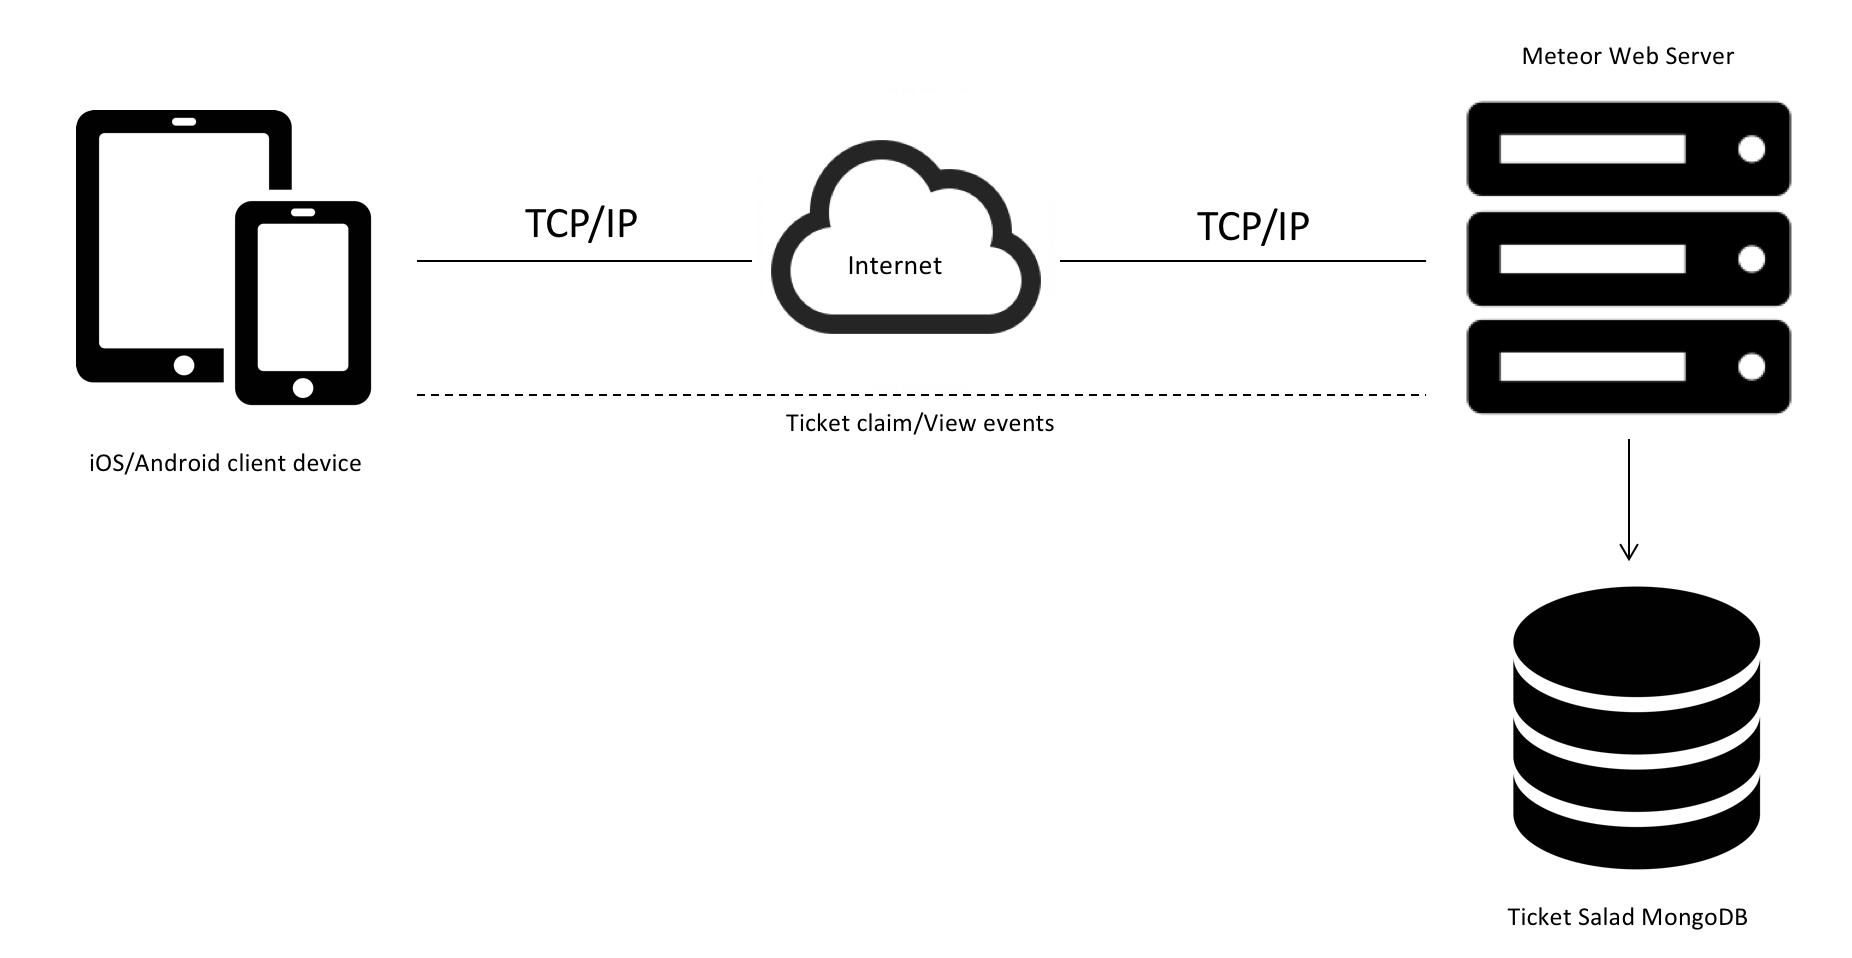
\includegraphics[width=\linewidth]{config.png}
	
	\section{Installation}
	
	The Ticket Salad application will be available on both iOS and Android platforms.
	For iOS users, the application will be available for download on the iOS App Store, while
	Android users will be able to download the application from the Google Play Store. Both iOS and Android 		users will undergo a similar process to install the application from their respective stores. Once the application 	has been found after searching, the user must simply tap the "install" button to install the application on their 	respective OS.
	
	\section{Getting Started}
	A user must have a Google account (for Android) or Apple ID (for iOS) in order to download the application
	from their respective stores. Once the application has been installed (See (3) Installation) and launched from
	their home screen, the user will be greeted with a screen that will give them the option to sign in if they have a  	pre-existing Ticket Salad account or create a new account. Once the user has successfully signed in, they will 
	be taken to the Ticket Salad home screen where all current event competitions will show with a burger-icon in the top right to access the main menu and a claim button at the bottom of the screen to make claims on a the respective event displayed.
	\\
	\\
	Tapping the burger-icon will show the app's main menu which serves as the main source of navigation through the app.
	
	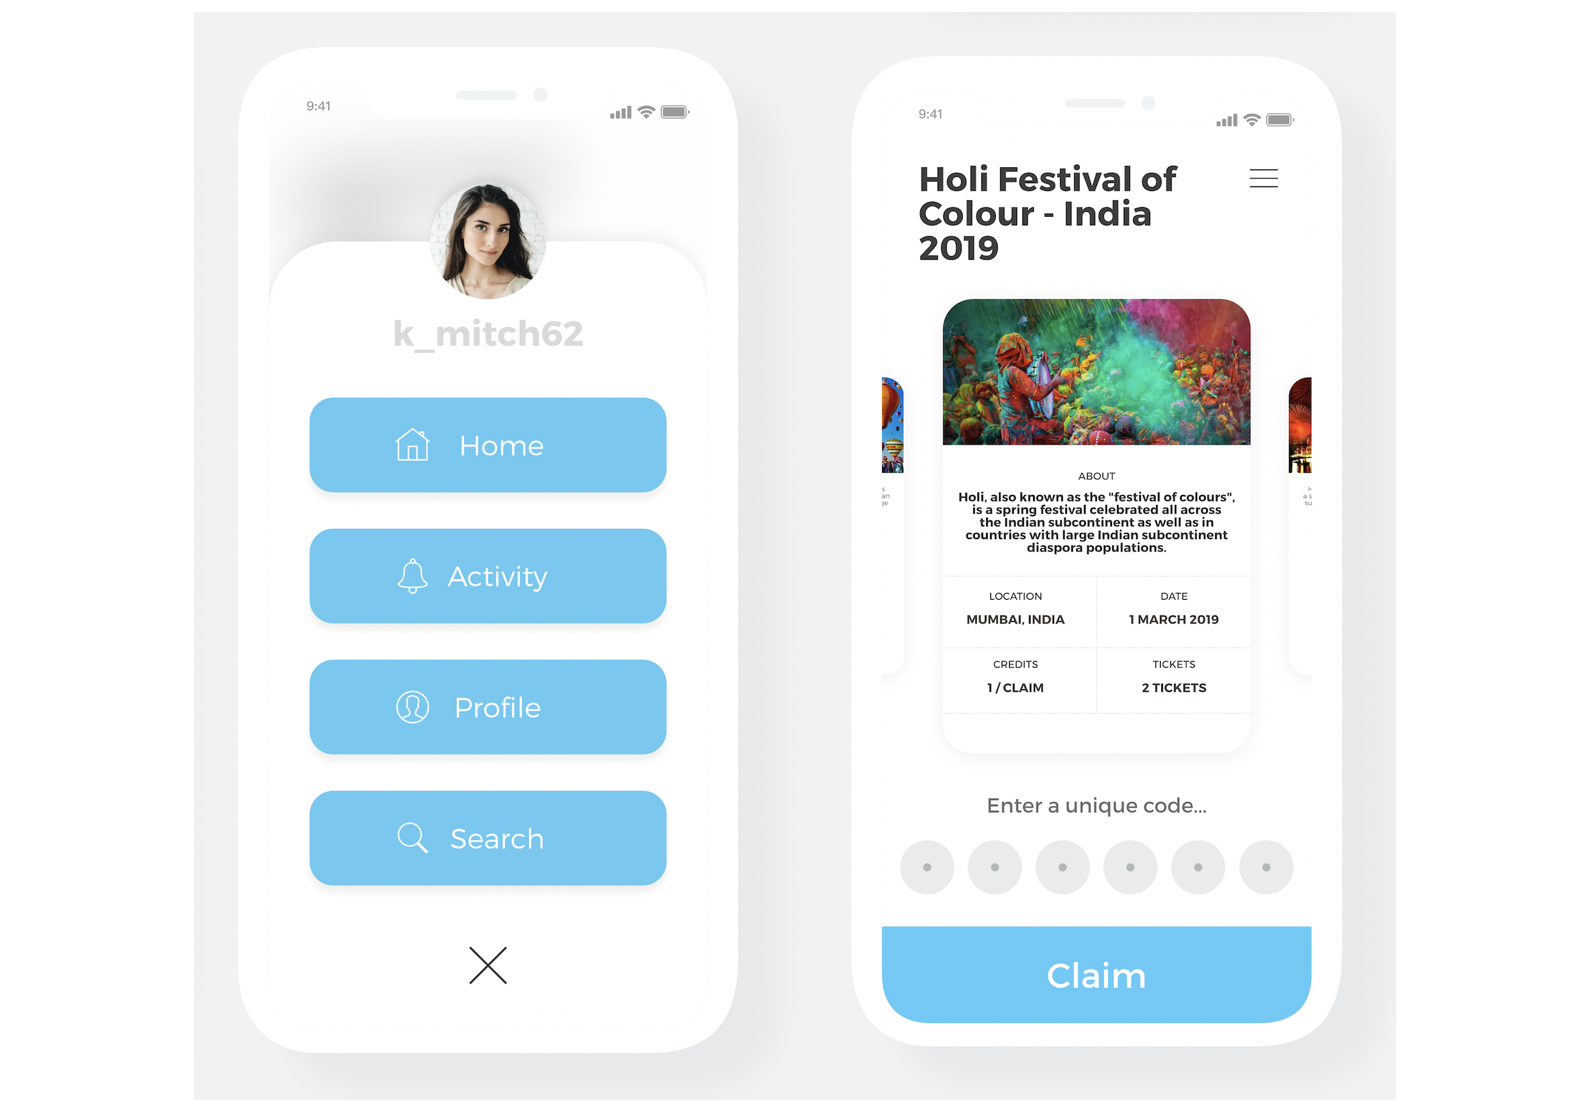
\includegraphics[width=\linewidth]{screens.png}

	\section{Using the system}
	\subsection{Signing Up}
	After opening the application, the user will land on the sign up screen (if they do not have an existing 		account) The user will then be required to enter in their details, making sure they use a valid email
	address. After all details have been added and are valid, the user will have to press the "Sign Up" button to 	create their Ticket Salad account. Once this is done, the user will land on the login page where their recently
	created details will have to be entered.
	\\
	\\
	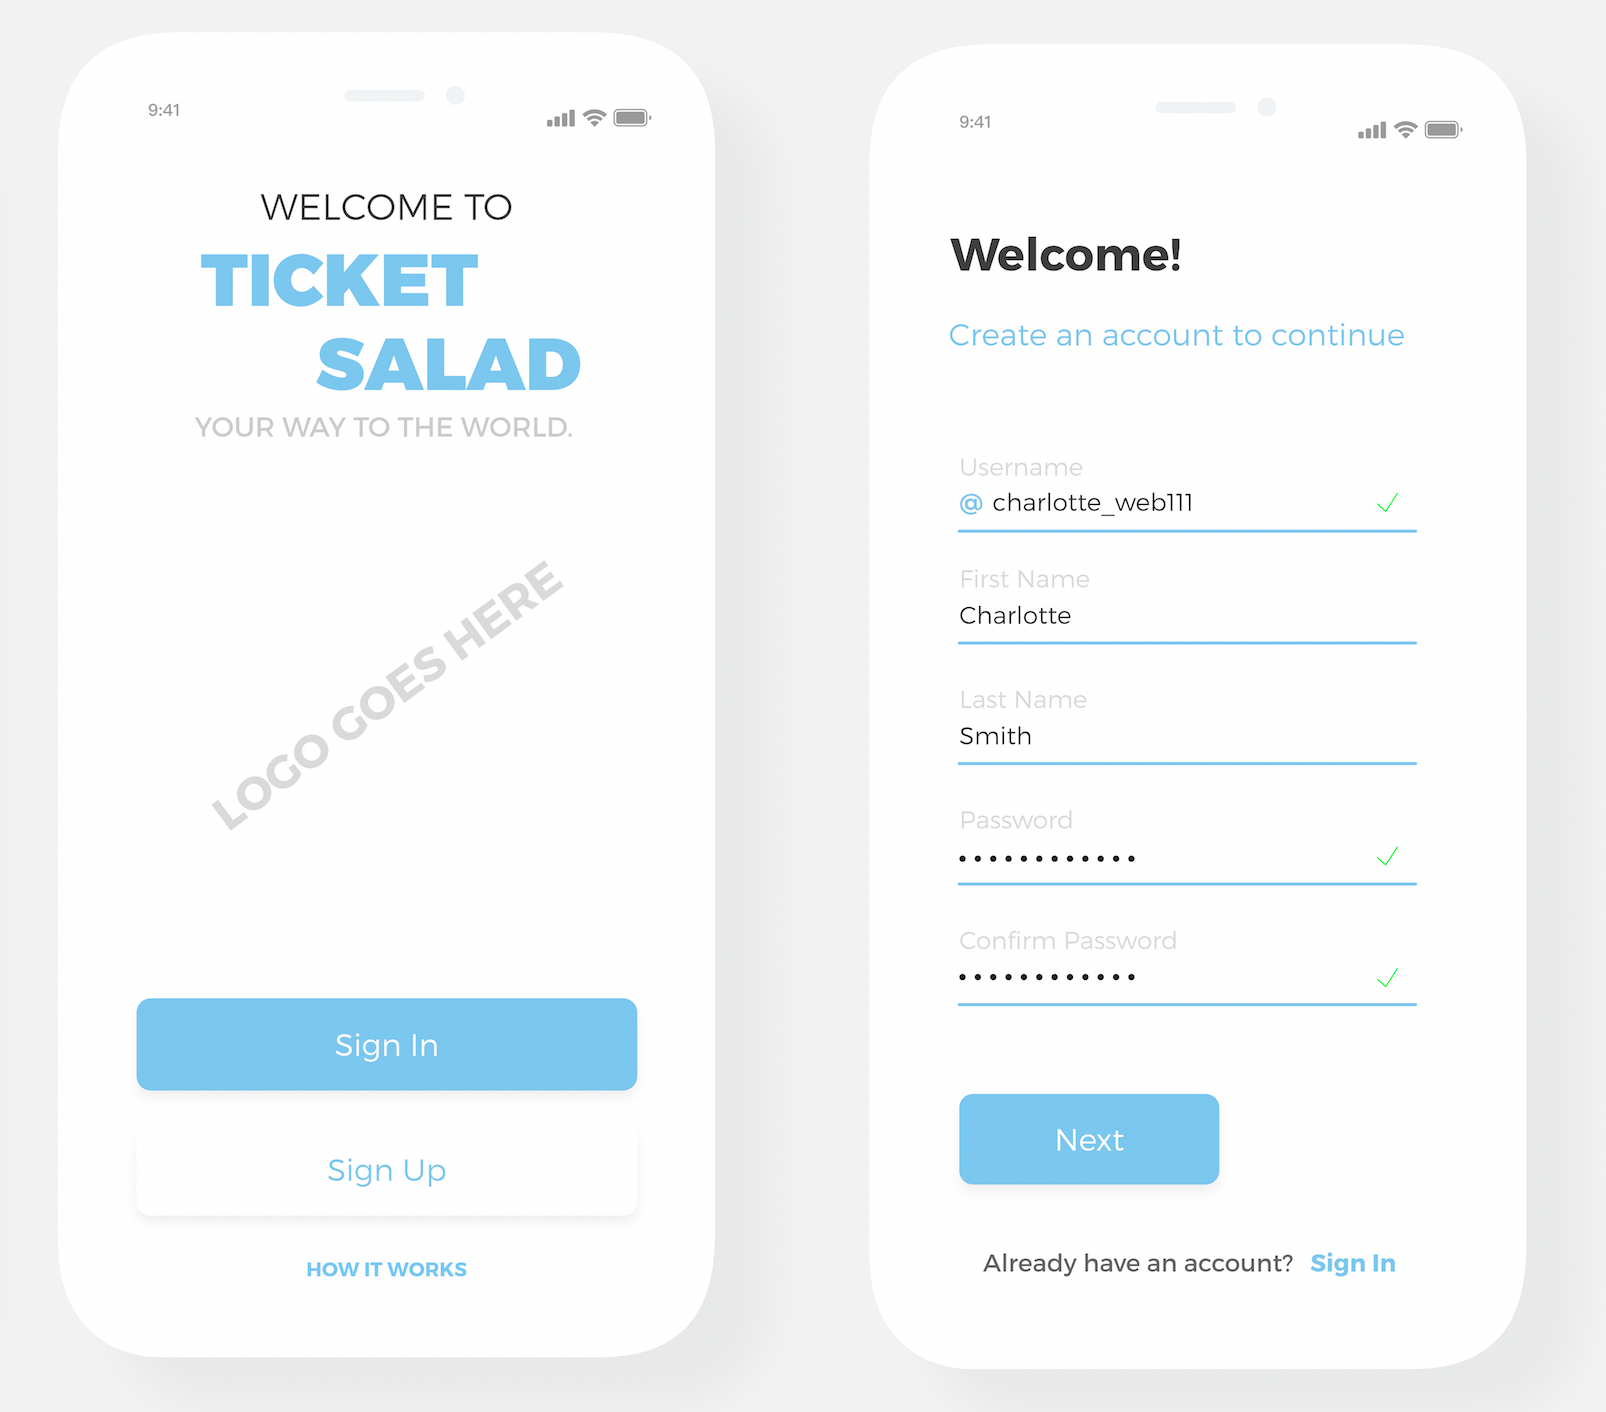
\includegraphics[width=\linewidth]{signup.png}
	\pagebreak

	\subsection{Logging In}
	Once the user has a valid account, they will be able to login to the app by specifying their
	email address and password and then tapping the "Sign In" button. The app will make a request
	to the Ticket Salad server to check if the details exist in the database, if the entered details are
	invalid or do not exist, the app will refuse the login request.
	\\
	\\
	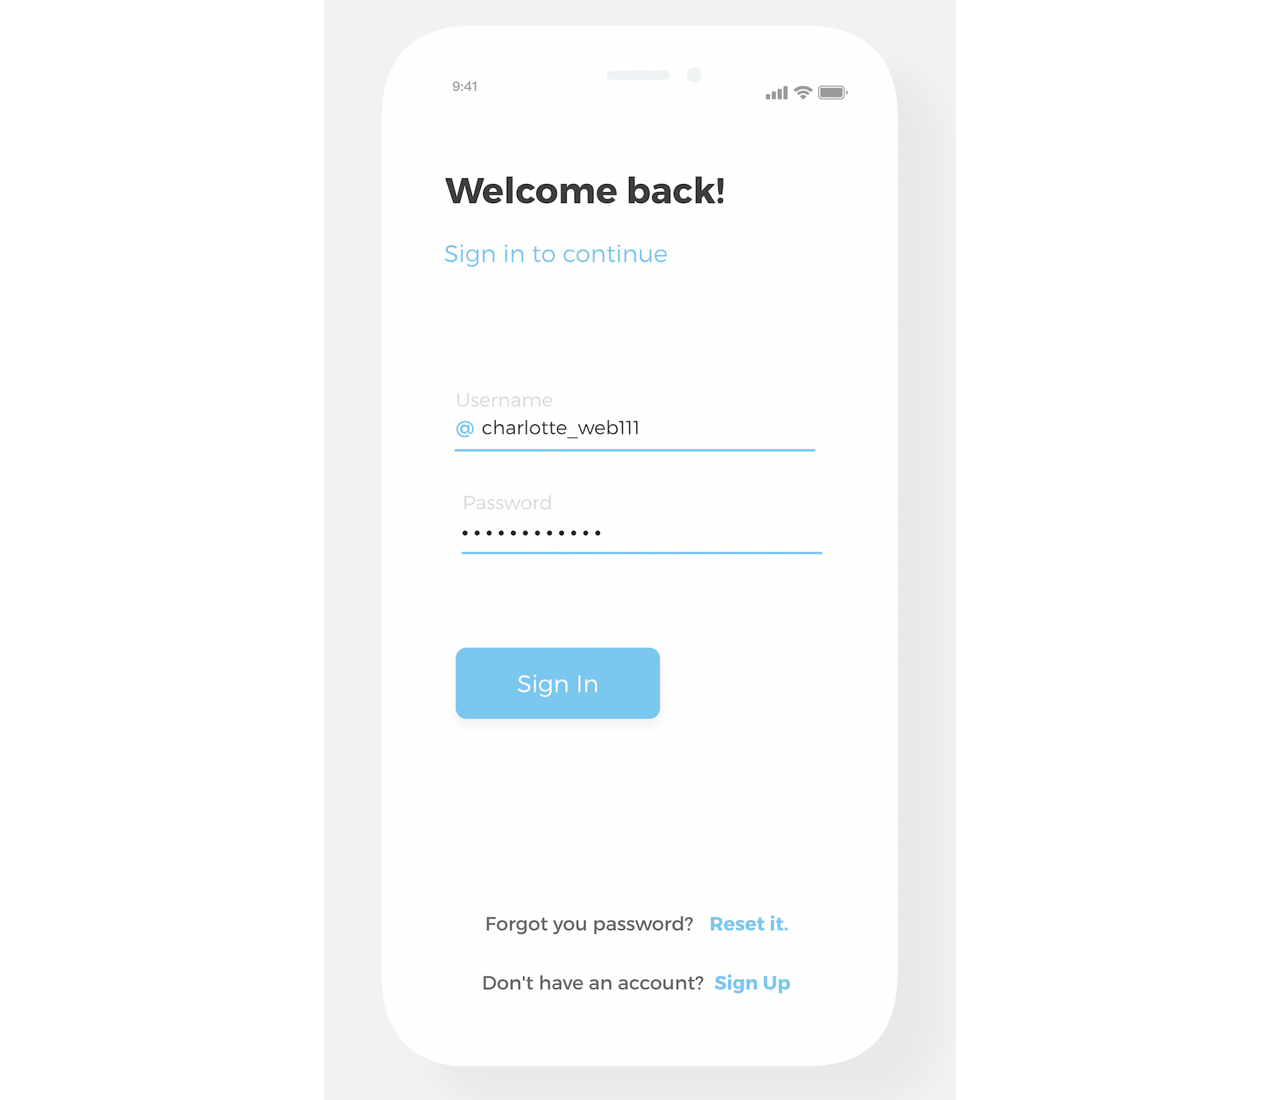
\includegraphics[width=\linewidth]{login.png}
	
	\subsection{Forgot Password}
	Should a registered user be unable to login due to a forgotten password, a
	forgotten password link is provided at the bottom of the login page. The user
	will use that link to reset their password by verifying their email.
	\pagebreak
	\subsection{Home screen and viewing/claiming events}
	Once the user has logged in, all current ticket events will be displayed in a carousel-styled view. The user can swipe through 
	the events and claim a bid on a ticket straight from this screen by entering a code and tapping the claim button located at the bottom of the screen. If the code is correct, a green screen will appear notifying the user that they have won and they will receive an email shortly, if the code is not correct, the user may try again provided they have sufficient claims.
	\\
	\\
	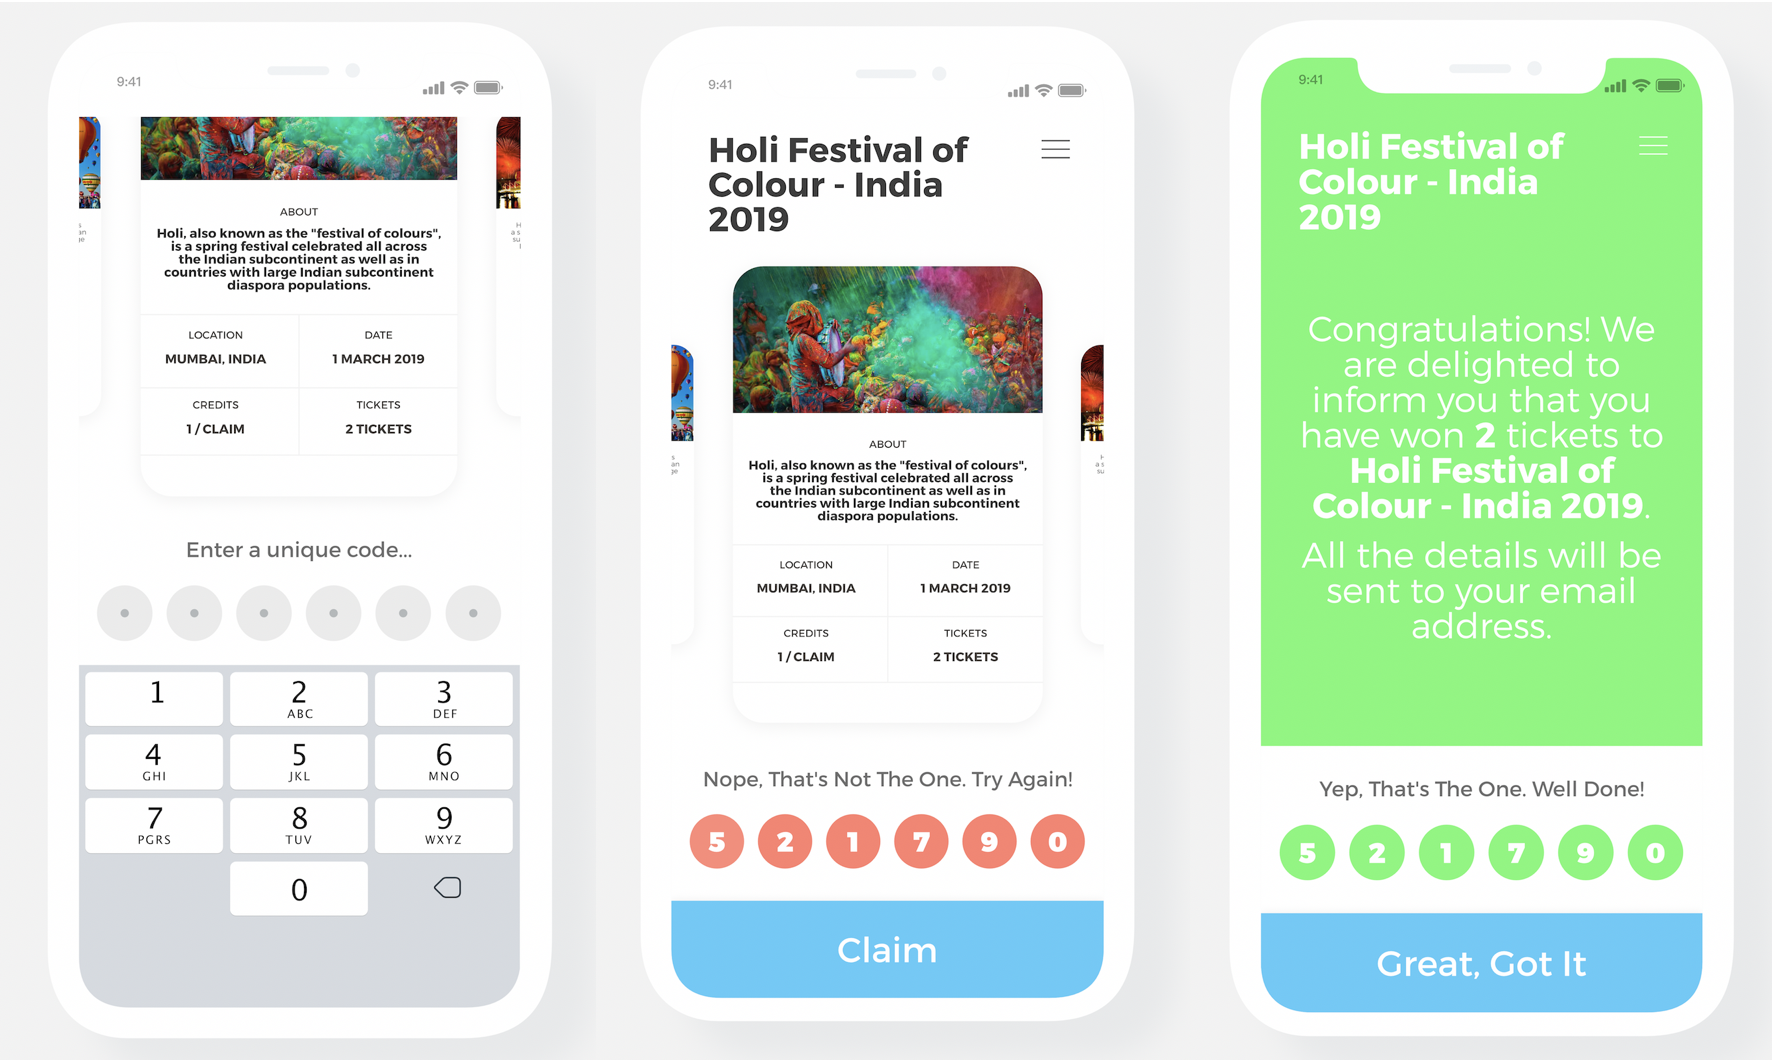
\includegraphics[width=\linewidth]{homescreen.png}
	\pagebreak
	\subsection{Profile}
	The profile page will allow the user to view their current details such as their profile picture, name and last name as well as their current in-app credit balance. The user can edit their profile, logout or buy more 		credits from this screen as well as access menus to help the user understand how the app works as well as contact Ticket Salad.
	\\
	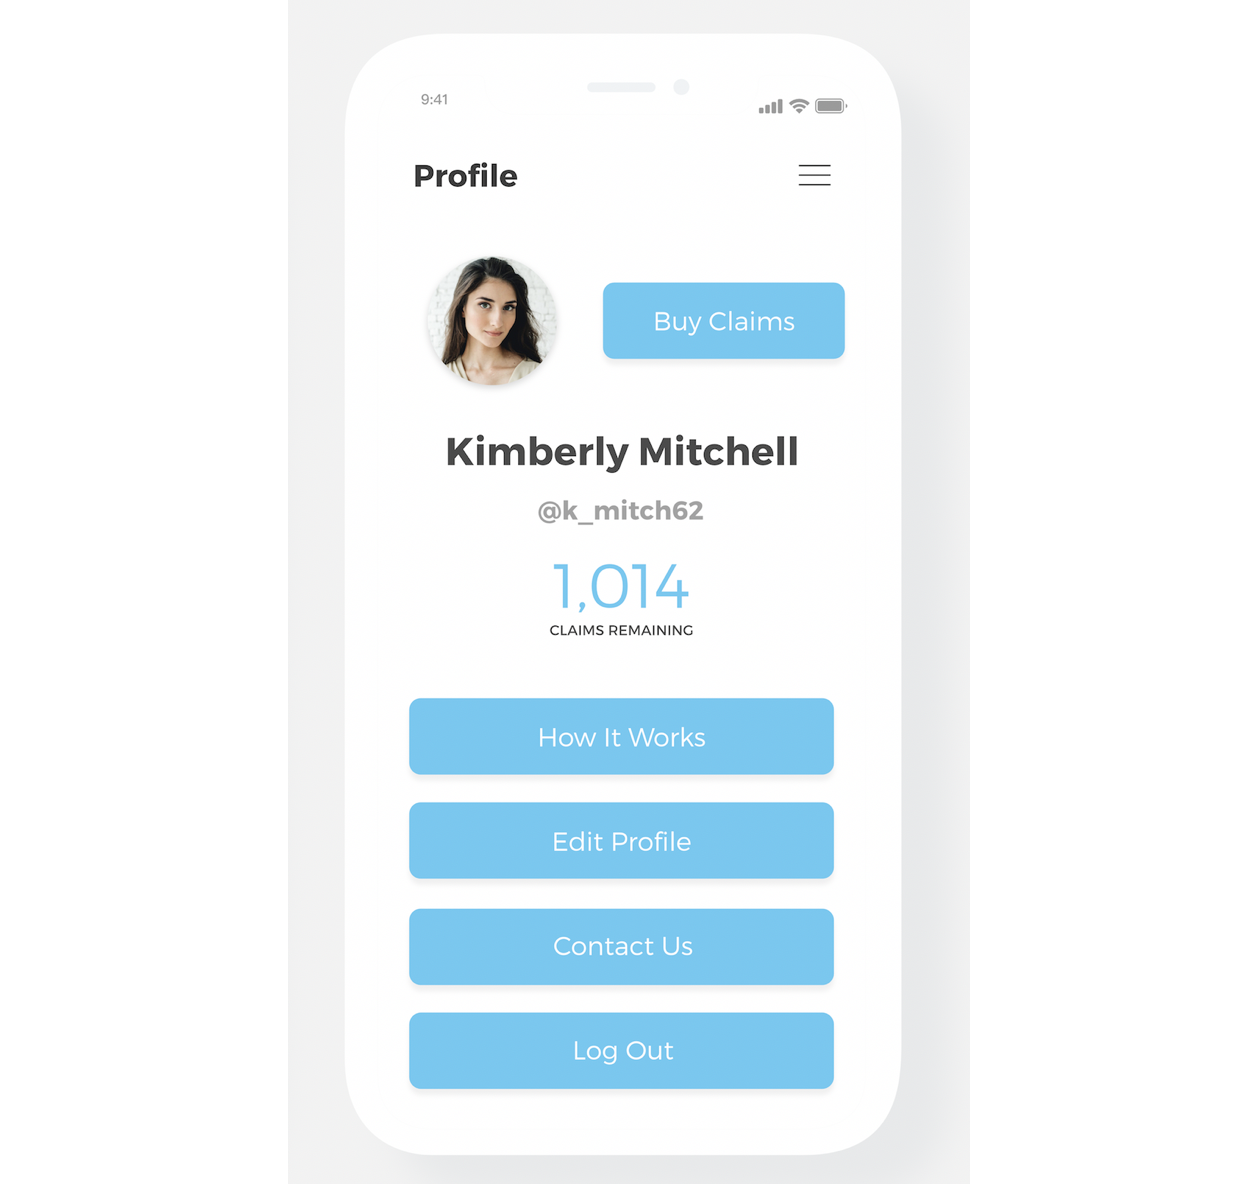
\includegraphics[width=\linewidth]{profile.png}
	\pagebreak
	\subsection{Edit Profile}
	This page allows the user to edit their current information provided the new information is valid, pressing 		"Save" will make a request to the Ticket Salad database to update the user's information.
	\\
	
\includegraphics[width=\linewidth]{edit.png}
	\pagebreak
	\subsection{Buy Credits}
	The Buy Credits screen is accessed through the user's profile and allows the user to buy more in-app credits
	to make ticket claims. Once the necessary payment authentication is done, the user's credit balance will 		update.
	\\
	\\
	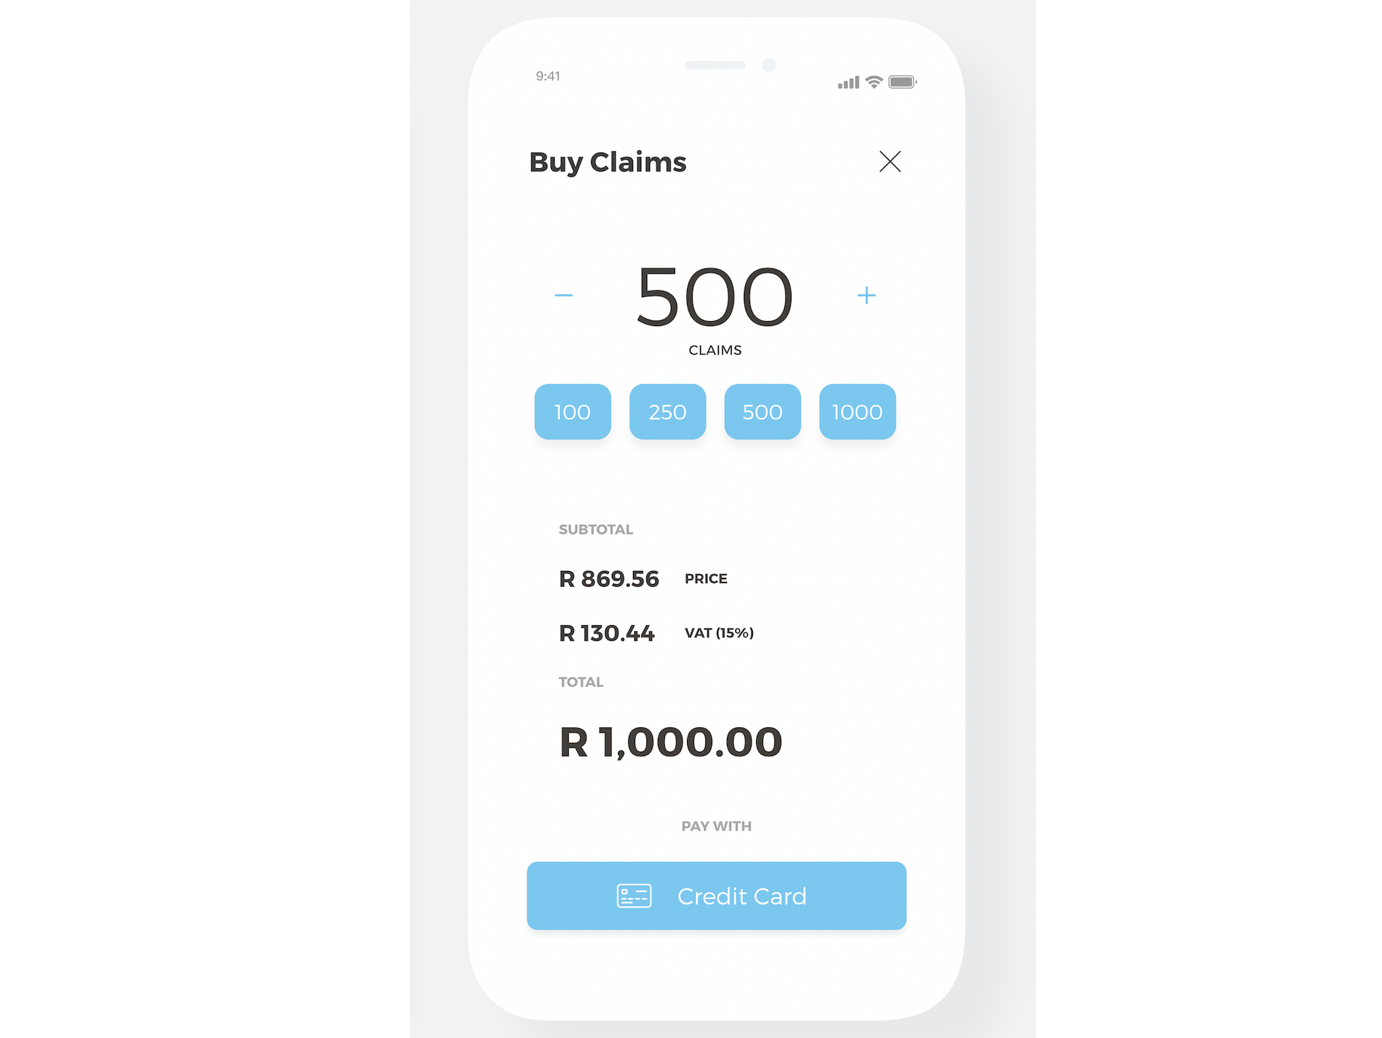
\includegraphics[width=\linewidth]{buy.png}
	\section{Troubleshooting}
	\subsection{Invalid Login Details}
	If a user is being denied access to the app through the login system, it is most likely due to an incorrect
	email and password combination. Tapping the "Forgot Password" link will allow the user to rest their password using their valid email address.
	\subsection{Insufficient Credits}
	If a user attempts to claim a ticket bid with insufficient credits, the app will not honour the bid. The user 
	must first top-up their credits through the "Buy Credits" page in order to make successful bids.
	\subsection{Server Downtime}
	In the event that server maintenance is required, possible server downtime will occur leaving all Ticket Salad 
	services offline. This downtime will be temporary and user's will be notified beforehand.
	
\end{document}




















